\chapter{Study Management}

 In this module the \entitylink{Study} aggregate is used to configure a
 study. It defines the valid types of specimens that can be collected, when
 they are to be collected from participants, and how the collected specimens
 are processed.

 This section first describes the study aggregate and then defines the commands
 it handles.

\section{Study Aggregate}

\begin{figure}[h]
  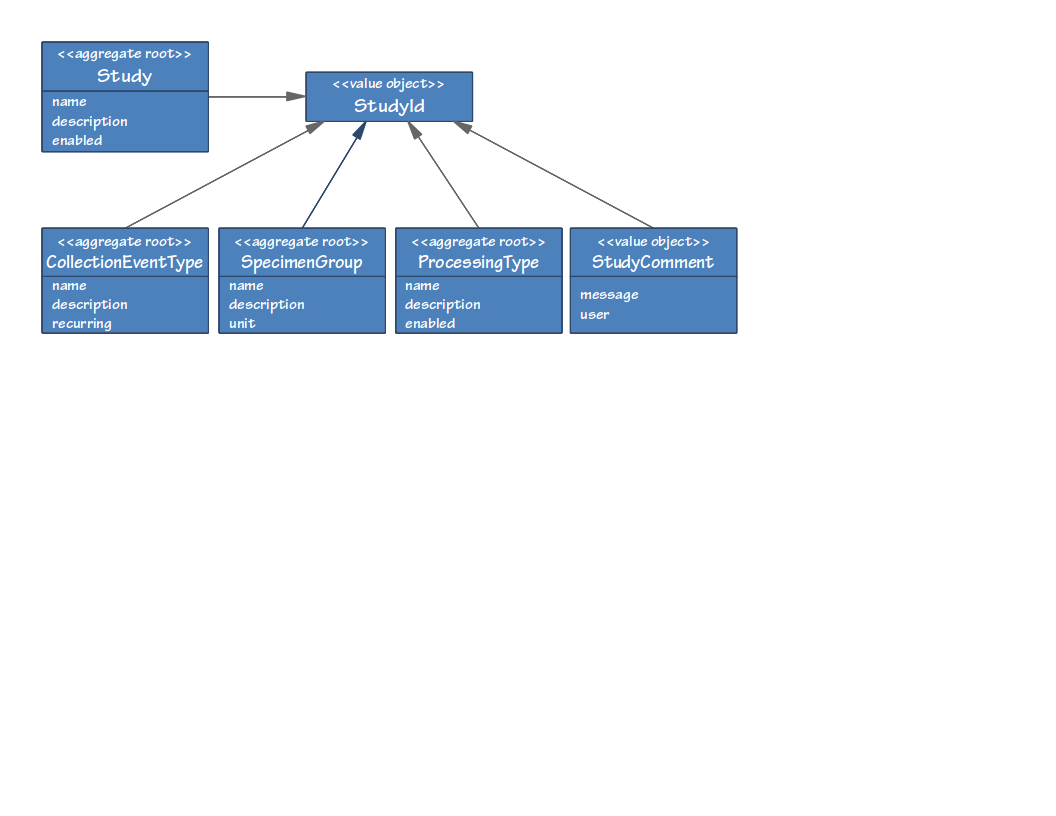
\includegraphics[trim={9mm 104mm 80mm 9mm}, clip,
    width=1\textwidth]{images/study-aggregate}
  \caption{Study aggregate}
  \label{fig:study-aggregate}
\end{figure}

\begin{description}[listparindent=\parindent]

  \item[\entitytarget{Study}] \hfill \\ Represents a collection of participants
    and specimens collected for a particular research study. The study name is
    a short descriptive name that is used to display summary information. The
    description contains text used to give more details on the name. Usually
    the name is an acronym and the description contains the words used in the
    acronym.

    A study can be enabled or disabled. When disabled, changes to its
    configuration are possible but patients and specimens cannot be added. When
    enabled, no further configuration changes are allowed, and participants and
    specimens can be added.

    A study may have one or more comments assigned to it during it's lifetime.

  \item[\entitytarget{SpecimenGroup}] \hfill \\ Ownership, summary, storage,
    and classification information that applies to an entire group or
    collection of \entitylink{Specimen}s.

    The anatomical source, preservation medium and specimen type are defined
    using other value objects discussed in Section \ref{sec:specimen-group}.

    This entity is used to record the specimen types used by the study. It can
    specify the specimens collected from participants, and the specimens that
    are processed from them.

  \item[\entitytarget{CollectionEventType}] \hfill \\ A classification name,
    unique to the \entitylink{Study}, for a visit by study participants. For
    specimen collection to be allowed on a study, at least one collection event
    type must be defined. Each collection event type has one or more specimen
    groups (see Section \ref{sec:collection-event-type}).

  \item[\entitytarget{ProcessingType}] \hfill \\ Describes a regularly
    performed specimen processing procedure with a unique name (unique to the
    \entitylink{Study}). There should be one or more associated
    \entitylink{SpecimenLinkType}s that (1) further define legal procedures and
    (2) allow recording of procedures performed on different types of
    \entitylink{Specimen}s.

  \item[\valobjtarget{StudyComment}] \hfill \\ The comment contains a message
    and the user that added the comment. The date and time the comment was made
    is recorded as meta data.

\end{description}

\subsection{SpecimenGroup}
\label{sec:specimen-group}

The SpecimenGroup entity is composed of other value objects as shown in Figure
\ref{fig:specimen-group}. \entitylink{SpecimenGroup} entities are accessed
via the \entitylink{Study} aggregate.

\begin{figure}[h]
  \centering
  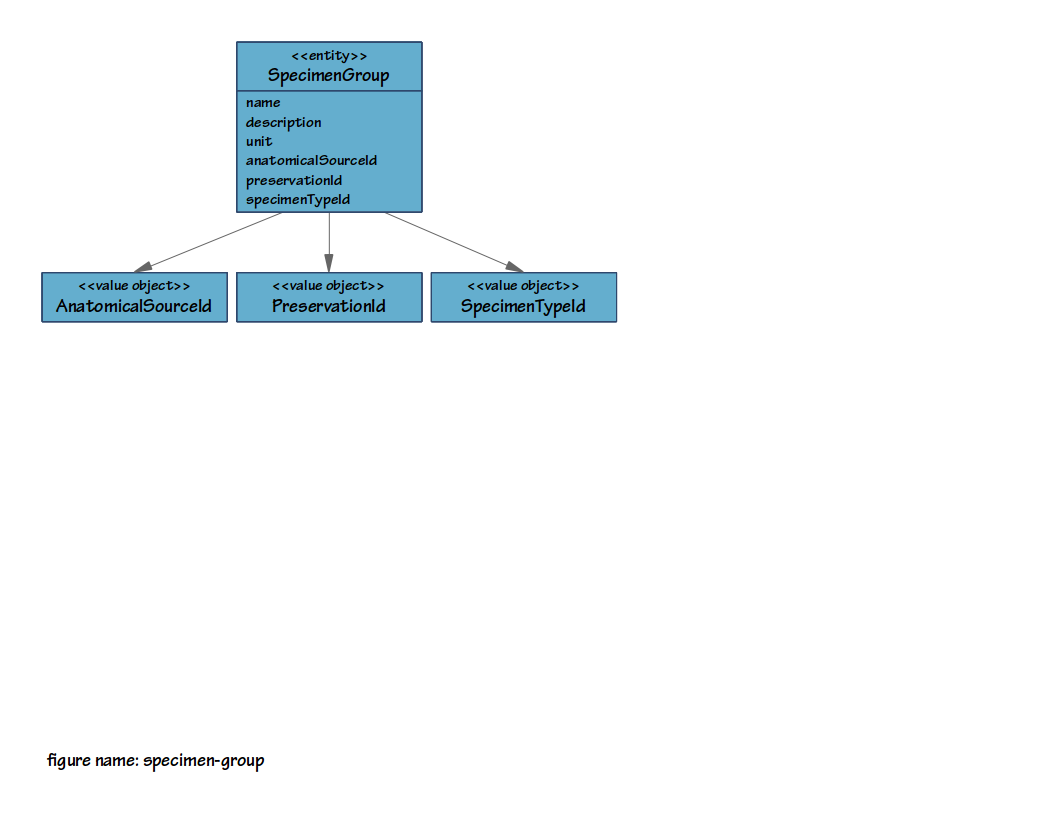
\includegraphics[trim={9mm 110mm 80mm 9mm}, clip,
    width=1\textwidth]{images/specimen-group}
  \caption{SpecimenGroup entity}
  \label{fig:specimen-group}
\end{figure}

\begin{description}

  \item[\valobjtarget{AnatomicalSource}] \hfill \\ A standardized set of
    regions of a \entitylink{Participant} \emph{where} a \entitylink{Specimen}
    is collected from. Potential examples include: colon, ear, leg, kidney,
    etc.

  \item[\valobjtarget{Preservation}] \hfill \\ Describes how a
    \entitylink{Specimen} should be preserved/stored by describing temperature
    requirements ($^\circ$C), as well as a preservation method (see
    \valobjlink{PreservationType}).

  \item[\valobjtarget{PreservationType}] \hfill \\ A standardized set of
    methods for preserving and storing \entitylink{Specimen}s.  Potential
    examples include: frozen specimen, RNA later, fresh specimen, slide, etc.

  \item[\valobjtarget{SpecimenType}] \hfill \\ A standardized set of
    classifications that describe \emph{what} a \entitylink{Specimen}
    is. Potential examples include: urine, whole blood, plasma, nail, protein,
    etc.

\end{description}

\subsection{CollectionEventType}
\label{sec:collection-event-type}

The \texttt{\textbf{\valobjtarget{SpecimenGroupCollectionEventType}}} value
object is used to define which types of specimens (i.e. which
\valobjlink{SpecimenGroup}s) need to be collected as part of a
\entitylink{CollectionEventType}. See Figure \ref{fig:collection-event-type}.

\begin{figure}[h]
  \centering
  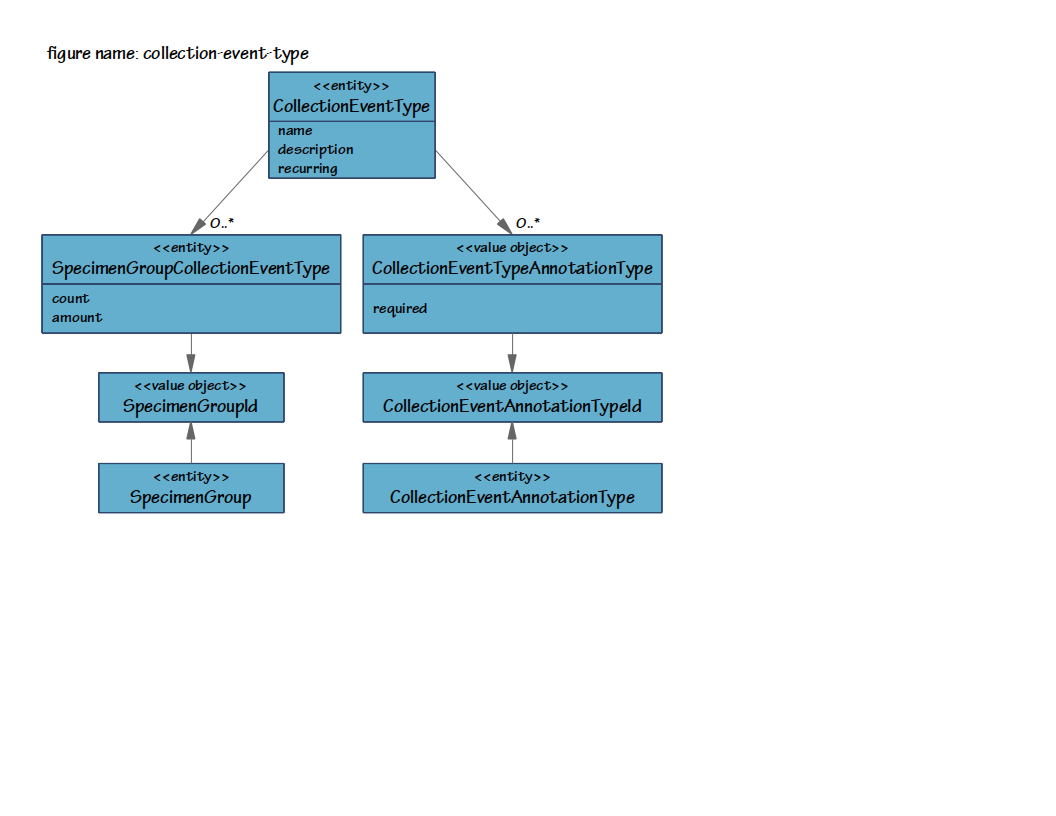
\includegraphics[trim={9mm 118mm 158mm 9mm}, clip,
    width=0.6\textwidth]{images/collection-event-type}
  \caption{Associating collection event types and specimen groups}
  \label{fig:collection-event-type}
\end{figure}

\subsection{ProcessingType}
\label{sec:Processing-type}

The \texttt{\textbf{\valobjtarget{SpecimenLinkType}}} represents a regularly
performed processing procedure involving two \entitylink{Specimen}s: an input,
which must be in a specific \valobjlink{SpecimenGroup}, and an output, which
must be in a specific \valobjlink{SpecimenGroup}.

The count specifies how many preservation types (e.g. tubes, FTA cards, etc.) are to
be collected. The amount is the volume required for each preservation type when
applicable. When not applicable the amount is set to zero.

\begin{figure}[h]
  \centering
  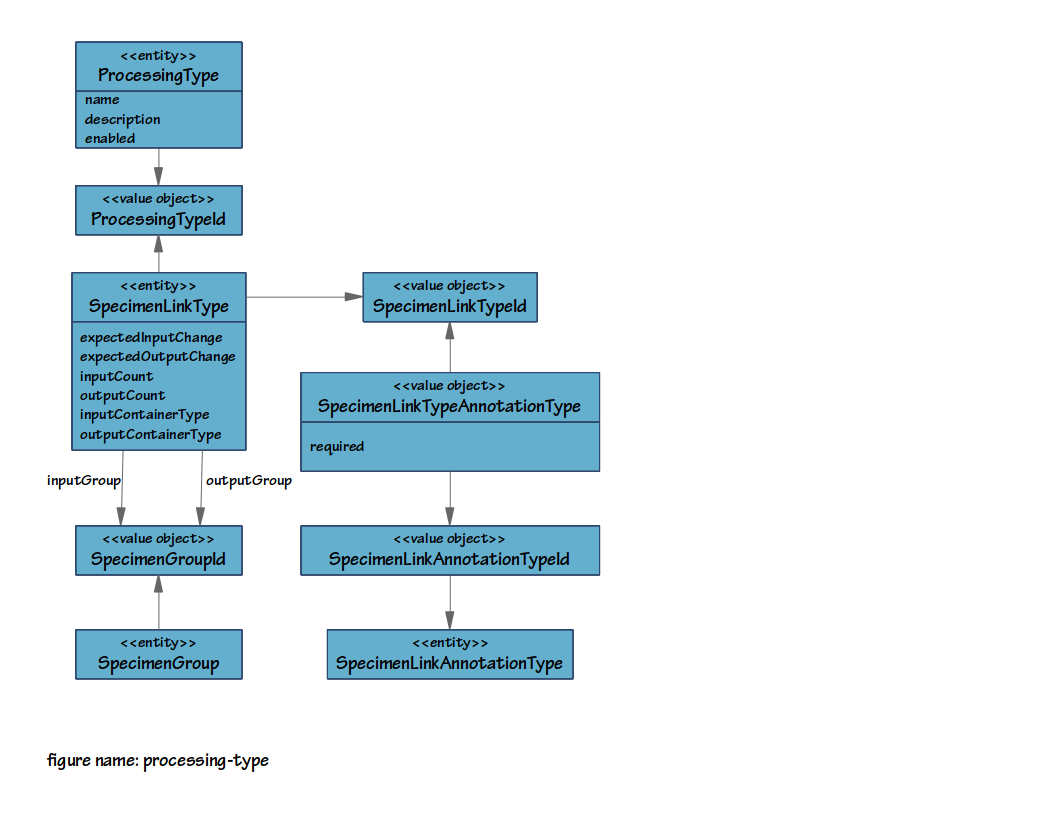
\includegraphics[trim={9mm 120mm 172mm 9mm}, clip,
    width=0.6\textwidth]{images/processing-type}
  \caption{Association processing types with specimen groups}
  \label{fig:processing-type}
\end{figure}

\section {Study Aggregate Commands}
